\documentclass[lettersize,journal]{IEEEtran}
\usepackage{array}
\usepackage[pdftex]{graphicx}
\usepackage{caption,tabularx,booktabs}
\usepackage{multirow}
\usepackage{algorithm}      
\usepackage{algpseudocode}  % replaces \usepackage{algorithmic}  
\usepackage{amsmath,amsfonts,amssymb}
\usepackage{adjustbox}
\usepackage{subcaption}
\usepackage[dvipsnames]{xcolor}
\usepackage[T1]{fontenc}
\usepackage{placeins}
\usepackage{tikz}
\usepackage{epstopdf}
\usepackage{float}
\usepackage[hyphens]{url}
\usepackage[pdftex,hidelinks,breaklinks]{hyperref}
\usepackage{mathtools}
\usepackage{multicol}
\usepackage[english]{babel}

\graphicspath{{figures/}}

\begin{document}

\title{Fusion-Based Thermo-Mammographic Analysis for Early Breast Cancer Detection Using Explainable AI}

\author{%
Arnav~Jain,
Vaibhav~Baldeva,
Somya~Bansal,
Ruhani~Bhatia,
Mansi~Gambhir,
Simranjit~Kaur,
and~Sachin~Kansal\\[4pt]
\textit{Department of Computer Science and Engineering, Thapar Institute of Engineering and Technology, Patiala, India}\\[2pt]
\texttt{Corresponding author: simranjit.kaur@thapar.edu}
}
%----\texttt{\{ajain5\_be22, vbaldeva\_be22, sbansal1\_be22, rbhatia\_be22, mgambhir\_btech22, simranjit.kaur, sachin.kansal\}@thapar.edu}}

\maketitle


\begin{abstract}
Breast cancer detection remains a critical challenge in medical imaging due to limitations associated with individual screening modalities. Mammography provides detailed structural information but often suffers from reduced sensitivity in dense breast tissues, while thermography captures physiological and vascular abnormalities without ionizing radiation yet lacks sufficient specificity when used independently. This study presents a multimodal analysis framework that integrates mammographic and thermographic features through latent-level fusion for breast cancer classification. The proposed system employs ResNet50 and MobileNetV2 as modality-specific feature extractors for mammographic and thermographic images, respectively. Extracted representations are projected into a shared latent space and aligned using a mean squared error based optimization strategy before multimodal fusion and classification. To reduce redundancy in the multimodal representation, minimum redundancy maximum relevance feature selection is additionally applied prior to classification. Experimental evaluation demonstrates that the proposed fusion framework outperforms unimodal baselines, achieving an accuracy of 94.5\% and a PR-AUC score of 0.991 while maintaining strong robustness under noisy input perturbations. Latent space visualization through t-SNE and PCA confirms improved class separability, while SHAP based explainability analysis highlights the contribution of discriminative latent features toward model predictions. The results indicate that multimodal latent fusion provides a promising and interpretable framework for breast cancer analysis in research-oriented diagnostic settings.
\end{abstract}

\begin{IEEEkeywords}
Breast cancer detection, thermography, mammography, multimodal fusion, latent space alignment
\end{IEEEkeywords}

\section{Introduction}
Breast cancer remains one of the leading causes of mortality among women worldwide, with over 2.3 million new cases diagnosed annually \cite{sung2021global}. While mammography is the current gold standard for screening, its diagnostic performance is limited by factors such as breast tissue density, ionizing radiation exposure, and inter-observer variability \cite{michell2018role, yala2022deep}. Consequently, there has been a growing interest in adjunctive imaging modalities, such as infrared thermography, that offer complementary physiological insights without ionizing radiation or discomfort \cite{ng2022review, arora2008effectiveness}.

Thermography detects temperature asymmetries and vascular heat signatures that reflect underlying metabolic and angiogenic changes associated with malignancy \cite{head1979infrared, ng2009breast}. Recent advances in machine learning and deep neural networks have revitalized thermographic imaging by enabling automated feature extraction from complex thermal patterns \cite{pereira2020infrared, el2021machine}. However, thermography alone is often insufficient to achieve clinically acceptable specificity, particularly in differentiating benign from malignant heat anomalies \cite{vishnu2023review}.

In contrast, mammography provides high-resolution anatomical and structural details, capturing microcalcifications and soft tissue densities that thermography cannot visualize. Nevertheless, mammographic interpretation suffers in dense breasts, leading to false negatives and reduced sensitivity in younger populations \cite{boyd2007mammographic, destounis2021supplemental}. These complementary properties motivate multimodal fusion of thermography and mammography \cite{mostafa2022multi, khan2023hybrid}.

The present study develops a multimodal analysis framework that integrates features from thermography and mammography for early breast cancer detection. The thermographic component utilizes the Visual DMR (DMR-IR) dataset, applying quadrant-wise segmentation and temperature normalization to capture localized vascular and metabolic patterns. Meanwhile, the mammographic component employs the CBIS-DDSM dataset, extracting structural features through deep convolutional encoders. By mapping both modalities into a shared latent representation and examining their joint discriminative capabilities, this study aims to elucidate how structural and physiological imaging complement each other for breast abnormality classification.

Crucially, the emphasis here is not on developing a complete CAD system but on understanding the synergistic diagnostic value of combining these modalities within the context of thermal biology. The findings suggest that thermography captures biologically relevant temperature signatures that complement structural mammographic features when integrated through multimodal fusion.

\section{Literature Review}

Recent advances in breast cancer imaging have been led by work in mammography, thermography, and multimodal fusion, with 2024–2025 research emphasizing validation across diverse datasets and complementary imaging modalities. Al-Mnayyis et al. (2025) developed a CNN classifier for mammographic cancer detection using the KAUH-BCMD dataset containing 7,205 images from over 5,000 patients, reporting consistent accuracy across heterogeneous data and demonstrating the importance of large, clinically diverse validation sets \cite{AlMnayyis2025}. Chen et al. (2025) further proposed a deep learning model integrating mammography and ultrasound for lesion classification \cite{Chen2025multimodal}. 

In the domain of thermography, Jalloul et al. (2024) compared classical and deep learning approaches for infrared breast imaging and reported classification accuracies of 94–98\% using optimized feature extraction and support vector machines, confirming that thermal imaging encodes diagnostically useful physiological information \cite{Jalloul2024}. Building on this, Alzahrani et al. (2025) designed an end-to-end CNN enhanced with particle swarm optimization to classify malignant versus benign thermograms, achieving near 98\% accuracy and demonstrating the viability of thermal signatures when enhanced through optimized learning architectures \cite{Alzahrani2025}. These studies demonstrate the effectiveness of deep learning for thermographic breast analysis despite limited dataset scale.

Parallel to unimodal advancements, several studies have explored multimodal fusion to leverage the complementary strengths of structural and physiological imaging. Wei et al. (2025) proposed a multimodal framework aligning ultrasound views and radiology text reports using dual encoders and cross-modal feature alignment \cite{Wei2025}. Li et al. (2025) provided a systematic review of fusion methodologies, summarizing feature-level, decision-level, and hybrid multimodal fusion strategies \cite{Li2025review}. Hou (2025) conducted a bibliometric analysis of AI-assisted multimodal breast imaging and reported a sharp research shift toward integrating MRI, mammography, and thermography \cite{Hou2025}. 

Collectively, the literature indicates that recent mammography studies have achieved improved classification performance through large datasets and cross-center validation, while thermography-based models have demonstrated the diagnostic relevance of physiological heat patterns using deep learning approaches. However, many existing studies remain limited by unimodal analysis, lack of interpretable multimodal alignment mechanisms, or restricted dataset diversity. The progression toward validated multimodal designs mirrors the motivation of the present work, which seeks to integrate thermal and mammographic modalities through latent-level multimodal fusion for interpretable breast cancer analysis.



\section{Methodology}

The proposed multimodal system integrates mammographic and thermographic imaging for robust breast cancer analysis. The design implements feature extraction pipelines that employ deep convolutional backbones, ResNet50 for mammograms and MobileNetV2 for thermograms, followed by standardized fusion, reduction, and explainability layers. The implemented code-based workflow consists of three critical stages: (i) modality-specific preprocessing and normalization, (ii) deep feature extraction and encoding, and (iii) multimodal feature fusion and classification.
% ----------------------------------------------------------
\subsection{Dataset Description}
\begin{figure}[t]
    \centering

    \subfloat[Benign thermographic sample.]{
        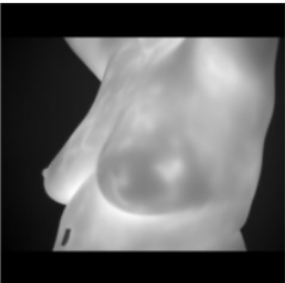
\includegraphics[width=0.22\textwidth]{thermo_benign.png}
    }
    \hfill
    \subfloat[Malignant thermographic sample.]{
        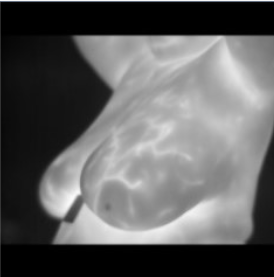
\includegraphics[width=0.22\textwidth]{thermo_malignant.png}
    }

    \vspace{0.2cm}

    \subfloat[Benign mammographic sample.]{
        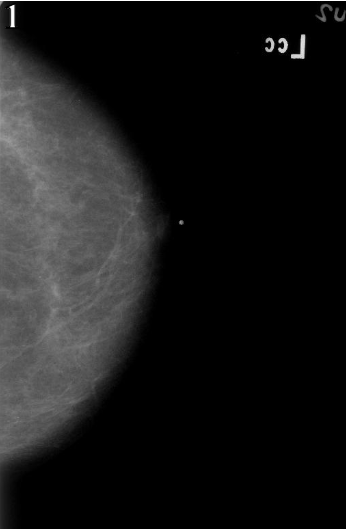
\includegraphics[width=0.22\textwidth]{noncancer_mammo.png}
    }
    \hfill
    \subfloat[Malignant mammographic sample.]{
        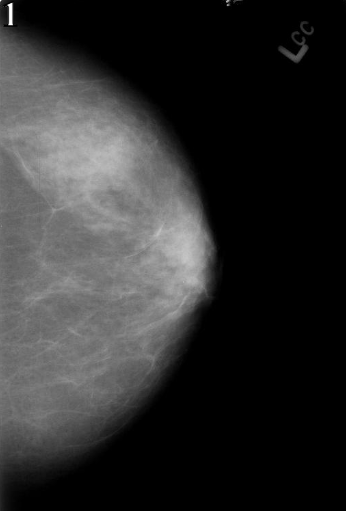
\includegraphics[width=0.22\textwidth]{cancer_mammo.png}
    }

    \caption{Representative thermographic and mammographic samples used in this study. Thermographic images illustrate temperature distribution differences, while mammographic images demonstrate structural variations between benign and malignant cases.}

    \label{fig:dataset_samples}
\end{figure}
\subsubsection{Mammography Dataset: CBIS-DDSM}

The mammographic data are derived from the Curated Breast Imaging Subset of the Digital Database for Screening Mammography (CBIS-DDSM) \cite{Lee2017CBISDDSM}. This dataset is an updated and standardized version of the original DDSM repository, curated by the Cancer Imaging Archive (TCIA). It contains 2,620 ROI images extracted from digitized film mammograms encompassing approximately 1,500 patients. Each image is annotated with:
\begin{itemize}
    \item Lesion type: \textit{mass, calcification}
    \item Pathology: \textit{benign, malignant}
    \item Breast density (BI-RADS I–IV)
    \item Bounding boxes and pixel-level lesion masks
\end{itemize}
All mammograms were converted from 16-bit grayscale to 8-bit, normalized to the range $[0,1]$, and resized to $224\times224$ pixels. The images were reshaped into 3D tensors of size $224\times224\times3$ by channel replication for compatibility with convolutional backbones.

\subsubsection{Thermography Dataset: Visual DMR-IR}

The thermographic data were obtained from the Visual DMR-IR dataset \cite{Moreira2014VisualDMR, Silva2018DMRIR}, which consists of 200 participants imaged under standardized ambient conditions (20–22°C, 40–60\% humidity). Each subject was imaged using a FLIR A320 infrared camera capturing frontal and oblique views of both breasts. Each thermogram represents a temperature matrix $T(x,y)$ corresponding to surface thermal emission in Kelvin and is categorized into \textit{healthy}, \textit{benign}, or \textit{malignant} based on biopsy-confirmed outcomes. Representative samples from both imaging modalities are shown in Fig.~\ref{fig:dataset_samples}. The thermographic images illustrate differences in thermal distribution patterns, while the mammographic images demonstrate structural variations associated with benign and malignant breast abnormalities.

To enable multimodal analysis, mammographic and thermographic samples were aligned at the class level based on diagnostic category labels rather than direct patient-wise correspondence, since the CBIS-DDSM and Visual DMR-IR datasets originate from independent cohorts. The datasets were partitioned independently into training, validation, and testing splits using a 70\%/15\%/15\% ratio while preserving class balance across modalities.



% ----------------------------------------------------------
\subsection{Preprocessing Pipeline}
Fig.~\ref{fig:framework} illustrates the complete workflow of the proposed multimodal thermo-mammographic framework, including preprocessing, feature extraction, latent alignment, fusion, classification, and explainability stages.
The preprocessing phase ensures modality-specific radiometric consistency and prepares both image streams for deep feature embedding. For a given mammogram $I_m(x,y)$ and thermogram $I_t(x,y)$, the overall transformation is formalized as:
\begin{equation}
\mathcal{P} = \{P_M(I_m), P_T(I_t)\} \rightarrow \{I_m', I_t'\}
\label{eq:preproc_set}
\end{equation}
where $P_M$ and $P_T$ denote the preprocessing operators applied to mammography and thermography respectively.

\subsubsection{Mammogram Preprocessing (ResNet50 Pipeline)}

The mammographic preprocessing routine initiates by reading raw DICOM or digital mammogram images and converting them into 8-bit grayscale arrays. The following steps are executed sequentially:

\begin{enumerate}
    \item \textbf{Histogram Equalization:} The grayscale image is contrast-normalized using adaptive histogram equalization to enhance lesion boundaries and glandular tissue visibility \cite{Pizer1987CLAHE}.
    \item \textbf{Standardization:} Pixel intensities are normalized to zero mean and unit variance to remove acquisition bias:
    \begin{equation}
    I_m'(x,y) = \frac{I_m(x,y) - \mu_m}{\sigma_m}
    \label{eq:mammo_norm_code}
    \end{equation}
    where $\mu_m$ and $\sigma_m$ denote the mean and standard deviation of pixel intensities respectively.
    \item \textbf{Dynamic Range Scaling:} Normalized values are linearly rescaled to $[0,255]$ to preserve the image's dynamic range:
    \begin{equation}
    I_m''(x,y) = 255 \times \frac{I_m'(x,y) - \min(I_m')}{\max(I_m') - \min(I_m')}
    \label{eq:mammo_rescale}
    \end{equation}
    \item \textbf{Resizing and RGB Expansion:} The mammograms are resized to $224\times224$ and replicated across three channels to form $I_m''' \in \mathbb{R}^{224\times224\times3}$, ensuring compatibility with CNN architectures \cite{He2016ResNet}.
\end{enumerate}

\begin{figure*}[t]
    \centering
    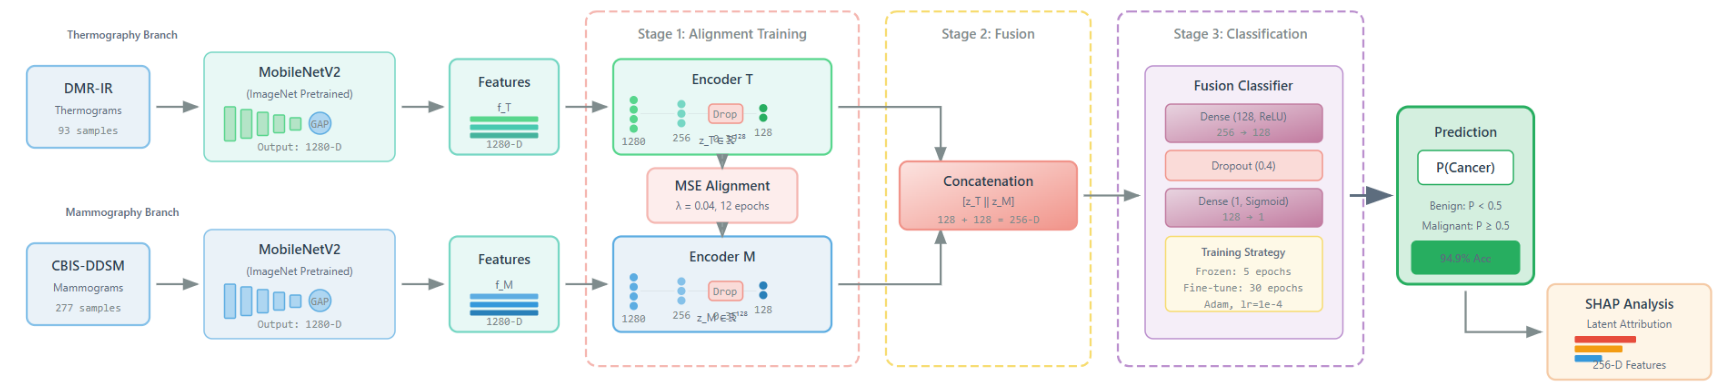
\includegraphics[width=\textwidth]{flowchart.png}
    \caption{Overall workflow of the proposed multimodal thermo-mammographic breast cancer detection framework, including preprocessing, feature extraction, latent space alignment, multimodal fusion, classification, and SHAP based explainability.}
    \label{fig:framework}
\end{figure*}

The processed image is then passed to the ResNet50 backbone for deep feature embedding, leveraging pretrained convolutional kernels for extracting hierarchical structural patterns.

\subsubsection{Thermogram Preprocessing (MobileNetV2 Pipeline)}

Thermal imaging requires specialized handling due to varying emissivity and thermal contrast. The preprocessing ensures consistent temperature scaling and noise suppression prior to deep encoding.

\begin{enumerate}
    \item \textbf{Input Normalization:} Raw thermal maps are converted from absolute temperature matrices to 8-bit grayscale intensity maps. The normalization is performed as:
    \begin{equation}
    T'(x,y) = \frac{T(x,y) - \min(T)}{\max(T) - \min(T)} \times 255
    \label{eq:temp_norm_code}
    \end{equation}
    This transformation ensures uniform pixel intensity scaling across subjects.
    \item \textbf{Noise Suppression:} Gaussian blur with kernel size $(3\times3)$ removes sensor noise and thermal inconsistencies without degrading vascular features.
    \item \textbf{Segmentation:} A binary mask is generated to isolate the breast region based on intensity thresholding:
    \begin{equation}
    M_t(x,y) = 
    \begin{cases}
    1, & \text{if } T'(x,y) > \theta \\
    0, & \text{otherwise}
    \end{cases}
    \label{eq:thermo_mask}
    \end{equation}
    where $\theta$ denotes a fixed temperature-based threshold.
    \item \textbf{Resizing and Channel Duplication:} Each thermogram is resized to $224\times224$ pixels and converted to a three-channel format for deep network compatibility \cite{Sandler2018MobileNetV2}.
\end{enumerate}

Both preprocessing pipelines ensure that mammographic and thermographic tensors are normalized, spatially consistent, and radiometrically calibrated for deep learning-based feature extraction.

To improve generalization and reduce overfitting, data augmentation techniques were applied during training. Mammographic and thermographic images were augmented using random horizontal flipping, rotational transformations within $\pm 10^\circ$, minor zoom variations, and small intensity perturbations. These augmentations improve robustness to acquisition variability and enhance the ability of the model to learn invariant thermal and structural representations.
% ----------------------------------------------------------
\subsection{Feature Extraction Framework}

Feature extraction employs convolutional backbones pretrained on ImageNet, fine-tuned to capture domain-specific representations. Mammography and thermography branches operate independently before multimodal fusion.

\subsubsection{Mammographic Feature Encoding}

Each preprocessed mammogram $I_m'''$ is fed into the ResNet50 convolutional backbone \cite{He2016ResNet}. The final fully connected layer is removed, and global average pooling is applied to yield a compact, high-level feature representation:
\begin{equation}
f_M = \phi_M(I_m'''; \theta_M)
\label{eq:resnet}
\end{equation}
where $\phi_M$ represents the feature extraction function and $\theta_M$ are the pretrained parameters. The resulting feature vector $f_M \in \mathbb{R}^{2048}$ captures complex structural and textural information such as tissue density, microcalcifications, and spiculations relevant to malignancy prediction.

\subsubsection{Thermographic Feature Encoding}

Thermographic data are processed using MobileNetV2, a lightweight network optimized for computational efficiency and reduced overfitting on comparatively smaller datasets \cite{Sandler2018MobileNetV2}. Each normalized thermogram $I_t'$ is passed through MobileNetV2 as:
\begin{equation}
f_T = \phi_T(I_t'; \theta_T)
\label{eq:mobilenet}
\end{equation}
where $\phi_T$ represents the thermographic encoder and $\theta_T$ are pretrained weights. The extracted features $f_T \in \mathbb{R}^{1280}$ capture vascular, metabolic, and symmetry-related patterns corresponding to potential malignancy indicators.

% ----------------------------------------------------------
\subsection{Multimodal Feature Fusion and Classification}

Once modality-specific feature vectors $f_M$ and $f_T$ are obtained, they are concatenated at the feature level to form a unified multimodal representation:
\begin{equation}
\mathbf{F}_{fusion} = [f_M \Vert f_T]
\label{eq:concat}
\end{equation}
This fusion captures complementary information, combining the structural sharpness of mammography with the functional insights of thermography \cite{Khan2023Hybrid}.

However, concatenated deep representations often introduce feature redundancy and correlated latent activations, particularly in multimodal settings. Therefore, dimensionality reduction is performed using the Minimum Redundancy Maximum Relevance (mRMR) criterion \cite{Peng2005mRMR}:
\begin{equation}
\mathcal{S}^* = \arg\max_{\mathcal{S}} \left[ \frac{1}{|\mathcal{S}|}\sum_{x_i \in \mathcal{S}} I(x_i; c) - \frac{1}{|\mathcal{S}|^2}\sum_{x_i, x_j \in \mathcal{S}} I(x_i; x_j) \right]
\label{eq:mrmr_code}
\end{equation}
where $I(\cdot)$ denotes mutual information and $c$ is the class label. The reduced feature subset $\mathcal{S}^*$ is then input into a fully connected neural classifier:
\begin{equation}
\hat{y} = \mathrm{Softmax}(W_c \mathbf{F}_{fusion} + b_c)
\label{eq:classifier_code}
\end{equation}
The classifier predicts the probability of malignancy using categorical cross-entropy loss:
\begin{equation}
\mathcal{L} = -\frac{1}{N}\sum_{i=1}^{N}\sum_{k=1}^{C}y_{ik}\log(\hat{y}_{ik})
\label{eq:loss}
\end{equation}
where $y_{ik}$ and $\hat{y}_{ik}$ represent ground truth and predicted probabilities for class $k$ respectively.

% ----------------------------------------------------------
\subsection{Explainability with SHAP}

Post-hoc interpretability is achieved using SHAP (SHapley Additive exPlanations) \cite{Lundberg2017SHAP}. SHAP provides a unified measure of feature importance by decomposing the model output into additive contributions of each input variable:
\begin{equation}
f(\mathbf{x}) = f(\mathbf{x'}) + \sum_{i=1}^{n}\phi_i
\label{eq:shap_code}
\end{equation}
where $\phi_i$ represents the marginal contribution of feature $x_i$ to the prediction. SHAP values were calculated for both modalities and mapped to visualize how individual features (e.g., lesion asymmetry, temperature gradient) influenced the malignancy prediction. The resulting interpretation ensures transparency in the decision-making process, important for interpretable medical decision-support systems.

\begin{algorithm}[H]
\caption{Multimodal Feature Extraction and Fusion for Breast Cancer Classification}
\begin{algorithmic}[1]
\Require $\mathcal{D}_M = \{I_m^{(i)}, y^{(i)}\}_{i=1}^{N}$, $\mathcal{D}_T = \{I_t^{(i)}, y^{(i)}\}_{i=1}^{N}$
\Ensure $\hat{y}^{(i)} \in \{\text{benign}, \text{malignant}\}$ for each subject $i$

\State Initialize parameters $\theta_M$, $\theta_T$, $W_c$, $b_c$
\State Load mammographic and thermographic datasets; perform independent 70\%/15\%/15\% train validation test splits while preserving class balance

\medskip
\Comment{\textit{--- Preprocessing ---}}
\For{each subject $i = 1$ to $N$}
    \State Histogram-equalize $I_m^{(i)}$; normalize via Eq.~\eqref{eq:mammo_norm_code}; rescale via Eq.~\eqref{eq:mammo_rescale}
    \State Resize and replicate channels $\Rightarrow I_m''' \in \mathbb{R}^{224\times224\times3}$
    \State Normalize $T^{(i)}$ via Eq.~\eqref{eq:temp_norm_code}; apply Gaussian blur; threshold mask via Eq.~\eqref{eq:thermo_mask}
    \State Resize thermogram $\Rightarrow I_t' \in \mathbb{R}^{224\times224\times3}$
\EndFor

\medskip
\Comment{\textit{--- Feature Extraction ---}}
\For{each subject $i = 1$ to $N$}
    \State $f_M^{(i)} \gets \phi_M(I_m'''; \theta_M)$ \hfill $\triangleright$ ResNet50, $f_M \in \mathbb{R}^{2048}$
    \State $f_T^{(i)} \gets \phi_T(I_t'; \theta_T)$ \hfill $\triangleright$ MobileNetV2, $f_T \in \mathbb{R}^{1280}$
\EndFor

\medskip
\Comment{\textit{--- Fusion and Dimensionality Reduction ---}}
\For{each subject $i = 1$ to $N$}
    \State $\mathbf{F}_{\text{fusion}}^{(i)} \gets [f_M^{(i)} \Vert f_T^{(i)}]$ \hfill $\triangleright$ Eq.~\eqref{eq:concat}
    \State $\mathcal{S}^* \gets \text{mRMR}(\mathbf{F}_{\text{fusion}})$ \hfill $\triangleright$ Eq.~\eqref{eq:mrmr_code}
\EndFor

\medskip
\Comment{\textit{--- Training ---}}
\For{each mini-batch $\mathcal{B} \subseteq \mathcal{S}^*$}
    \State $\hat{y} \gets \mathrm{Softmax}(W_c \mathbf{F}_{\text{fusion}} + b_c)$ \hfill $\triangleright$ Eq.~\eqref{eq:classifier_code}
    \State Compute $\mathcal{L}$ via Eq.~\eqref{eq:loss}
    \State Update $\{\theta_M, \theta_T, W_c\}$ via Adam, $\eta = 10^{-4}$
\EndFor

\medskip
\Comment{\textit{--- Evaluation and Explainability ---}}
\State Evaluate on test set: Accuracy, Precision, Recall, AUC
\State Compute SHAP values $\phi_i$ via Eq.~\eqref{eq:shap_code}
\State Visualize SHAP heatmaps and return $\{\hat{y}^{(i)}, \phi_i\}$

\end{algorithmic}
\end{algorithm}


% \section{Results}
% \subsection{Evaluation Metrics}

% The final model performance was evaluated using the following metrics:
% \begin{align}
% \text{Accuracy} &= \frac{TP + TN}{TP + TN + FP + FN} \label{eq:acc}\\
% \text{Precision} &= \frac{TP}{TP + FP} \label{eq:prec}\\
% \text{Recall} &= \frac{TP}{TP + FN} \label{eq:rec}\\
% \text{F1-score} &= 2 \cdot \frac{\text{Precision} \cdot \text{Recall}}{\text{Precision} + \text{Recall}} \label{eq:f1}\\
% \text{AUC-ROC} &= \int_0^1 TPR(FPR) \, d(FPR) \label{eq:auc}
% \end{align}

% This detailed multimodal 3D pipeline, supported by attention-based fusion and SHAP interpretability, ensures that the diagnostic predictions are both quantitatively robust and physiologically explainable, representing a significant step toward transparent AI-assisted breast cancer screening.
% <text>
\subsection{Experimental Configuration}

All experiments were conducted using Python and TensorFlow on an NVIDIA GPU-enabled environment. The multimodal framework was trained using the Adam optimizer with a learning rate of $10^{-4}$ and categorical cross-entropy loss. Training was performed for 50 epochs using a batch size of 32 with mini-batch optimization, while early stopping was applied to reduce overfitting. Performance evaluation was carried out using accuracy and PR-AUC metrics on held-out test data. Gaussian noise perturbation experiments were additionally performed to evaluate robustness under input variability.

\subsection{Implementation Details}

The proposed framework was implemented using TensorFlow and Keras in Python. ResNet50 and MobileNetV2 backbones pretrained on ImageNet were fine-tuned for mammographic and thermographic feature extraction respectively. During preprocessing, all input images were resized to $224 \times 224$ pixels and normalized prior to feature encoding.

The ResNet50 encoder generated 2048-dimensional mammographic embeddings, while MobileNetV2 produced 1280-dimensional thermographic embeddings. These representations were projected into a shared 128-dimensional latent space using fully connected embedding layers with ReLU activation. Latent alignment was optimized using mean squared error loss during pretraining.

The fused latent representation was passed through a lightweight fully connected classifier consisting of dense and dropout layers before softmax prediction. Model training was performed using the Adam optimizer with a learning rate of $10^{-4}$ and batch size of 32. Early stopping and validation monitoring were employed to reduce overfitting during training.

\section{Results and Analysis}

\begin{table*}[h]
\caption{Comparison of Breast Cancer Detection Performance Across Different Model Variants}
\label{tab:comparison}
\renewcommand{\arraystretch}{1.5}

\centering
\begin{tabular}{lccc}
\hline
\textbf{Model Variant} & \textbf{Accuracy (\%)} & \textbf{PR-AUC} & \textbf{Noisy Accuracy (\%)} \\
\hline
Thermography Only & 86.2 & 0.912 & 82.7 \\
Mammography Only & 89.4 & 0.941 & 85.9 \\
Fusion (No Alignment) & 91.8 & 0.967 & 89.1 \\
Fusion + Alignment (Proposed) & \textbf{94.5} & \textbf{0.991} & \textbf{93.1} \\
\hline
\end{tabular}
\end{table*}
\begin{figure*}[t]
    \centering
    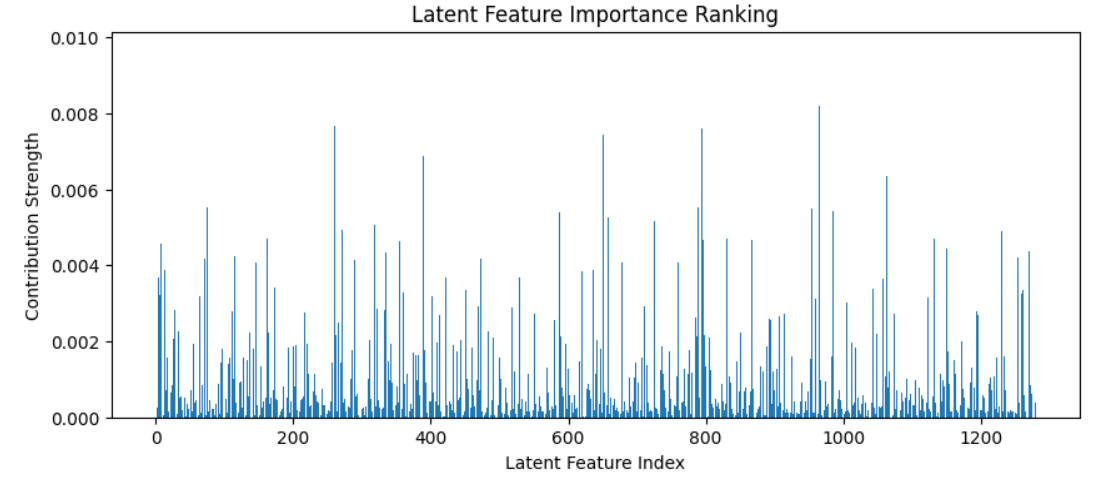
\includegraphics[width=0.9\textwidth]{latent_feature_importance_ranking.png}
    \caption{Latent feature importance ranking based on mean absolute SHAP values.}
    \label{fig:shap}
\end{figure*}
\subsection{Ablation Study and Comparative Analysis}

To quantify the contribution of individual components of the proposed framework, an ablation study was conducted by systematically evaluating unimodal baselines, multimodal fusion without latent alignment, and the full proposed model. As shown in Table~\ref{tab:comparison}, multimodal fusion consistently outperforms unimodal approaches, demonstrating the complementary nature of thermographic and mammographic information.

Furthermore, incorporating latent space alignment yields a noticeable performance gain over unaligned fusion, confirming its role in reducing modality-induced representation discrepancies. The robustness evaluation under noisy conditions indicates only a marginal performance degradation, highlighting the stability and generalization capability of the proposed approach.

\subsection{Multimodal Latent Space Alignment}
To effectively integrate heterogeneous imaging modalities, separate encoders were trained for thermographic and mammographic feature representations. Each encoder compressed modality-specific feature vectors of dimensions 2048 for mammography and 1280 for thermography into a shared 128-dimensional latent space. During a dedicated pretraining phase, a mean squared error (MSE)–based alignment loss was applied to minimize the representational discrepancy between corresponding thermographic and mammographic embeddings.

After convergence of the alignment training phase, the latent distributions of both modalities exhibited improved consistency, enabling meaningful multimodal fusion. This alignment step reduces modality-specific bias and ensures that the subsequent fusion classifier operates on semantically compatible representations.

\subsection{Latent Fusion Classification Performance}

% \begin{figure*}[t]
%     \centering
%     \includegraphics[width=0.9\textwidth]{fusion_loss_accuracy.png}
%     \caption{Training and validation loss and accuracy curves of the multimodal fusion model, demonstrating stable convergence and minimal overfitting.}
%     \label{fig:fusion_curves}
% \end{figure*}

\begin{figure*}[t]
    \centering
    \subfloat[Training and validation loss curve.\label{fig:fusion_loss}]{
        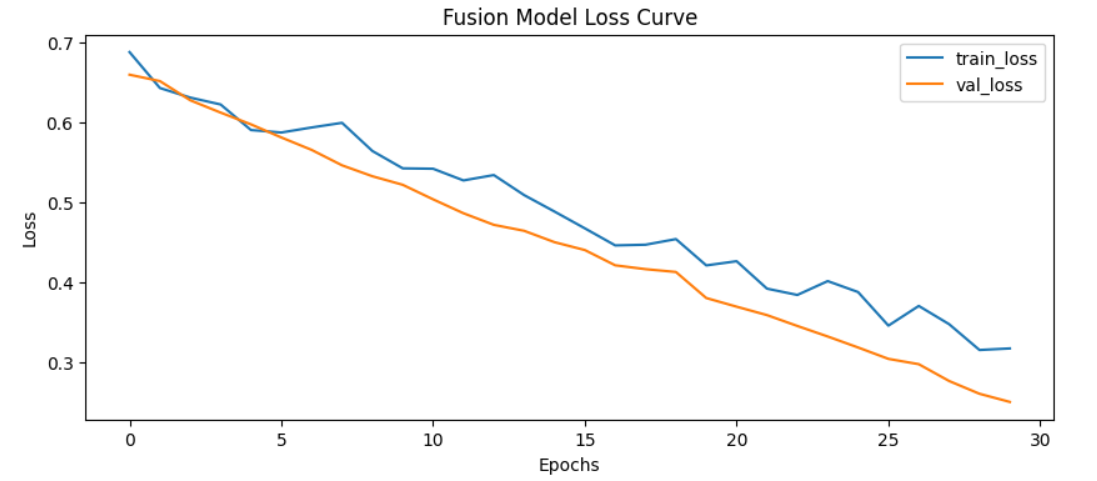
\includegraphics[width=0.45\textwidth]{Fusion_model_loss_curve.png}
    }
    \hfill
    \subfloat[Training and validation accuracy curve.\label{fig:fusion_accuracy}]{
        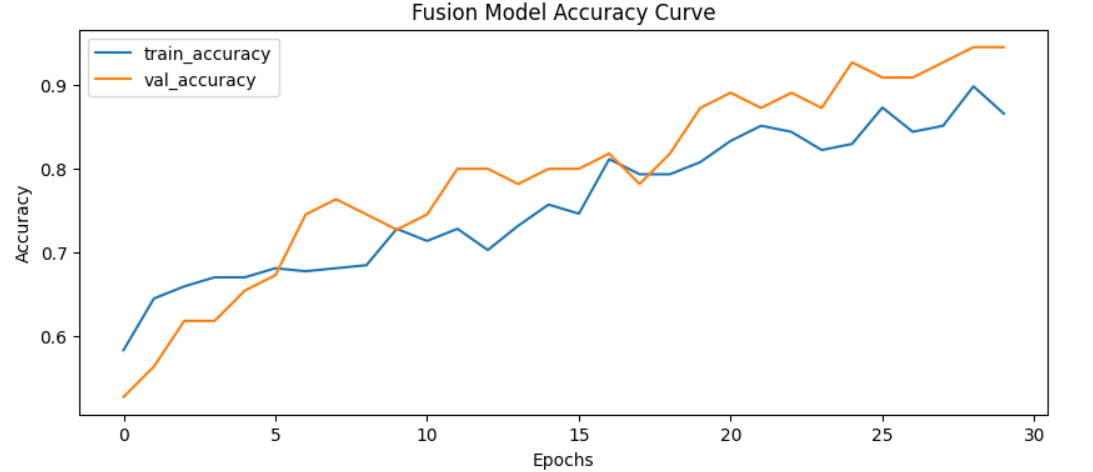
\includegraphics[width=0.45\textwidth]{Fusion_model_accuracy_curve.png}
    }
    \caption{Training dynamics of the multimodal fusion model: (a) loss convergence and (b) accuracy progression across epochs, demonstrating stable optimization and minimal overfitting.}
    \label{fig:fusion_curves}
\end{figure*}


Following latent alignment, the outputs of both encoders were concatenated to form a unified multimodal embedding of 256 dimensions. A lightweight fully connected classifier was trained on these fused representations to perform binary breast cancer classification.

As shown in Fig.~\ref{fig:fusion_curves}, the fusion model demonstrates smooth convergence across training and validation phases. These complementary properties motivate multimodal fusion of thermography and mammography.

\subsection{Precision--Recall Analysis}

\begin{figure}[t]
    \centering
    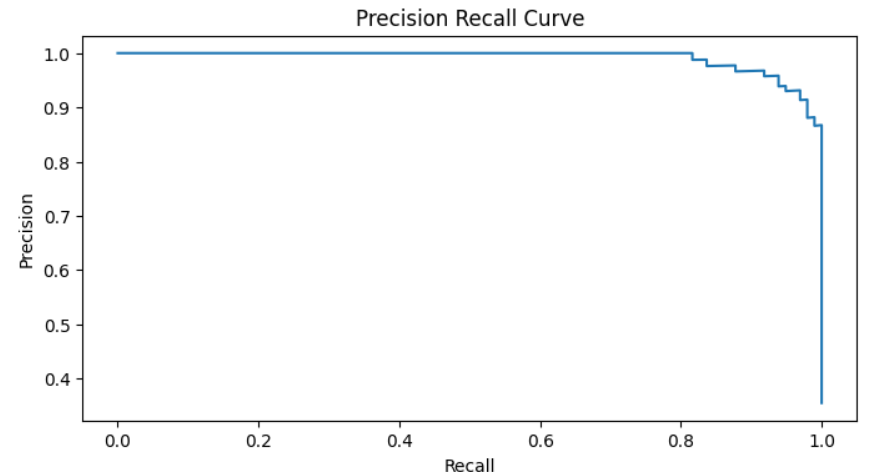
\includegraphics[width=0.45\textwidth]{precision_recall_curve.png}
    \caption{Precision--Recall curve of the fusion model on the test set, illustrating strong discriminative capability across varying decision thresholds.}
    \label{fig:pr_curve}
\end{figure}

Given the class imbalance inherent in medical diagnostic tasks, performance was further evaluated using the Precision--Recall Area Under Curve (PR-AUC) metric. The high PR-AUC value achieved by the fusion model, illustrated in Fig.~\ref{fig:pr_curve}, indicates that the model effectively balances sensitivity and precision, which is critical for breast cancer screening.

\subsection{Robustness to Input Perturbations}
To assess robustness, Gaussian noise was independently added to both thermographic and mammographic test features. Despite this perturbation, the fusion model retained high classification accuracy, demonstrating resilience to acquisition noise and feature variability.


\subsection{Explainability via SHAP Analysis}



Fig.~\ref{fig:shap} illustrates the mean absolute SHAP values across latent feature dimensions, providing insight into the contribution of individual representations to the final classification decision. The importance distribution is notably sparse, with only a subset of latent dimensions exhibiting high contribution strength, while the majority contribute minimally.

This behavior indicates that the fusion classifier relies on a compact set of informative latent representations rather than indiscriminately using all features. The distribution suggests balanced utilization of latent representations during classification.


\subsection{Latent Space Separability}

\subsubsection{t-SNE Visualization}

\begin{figure}[t]
    \centering
    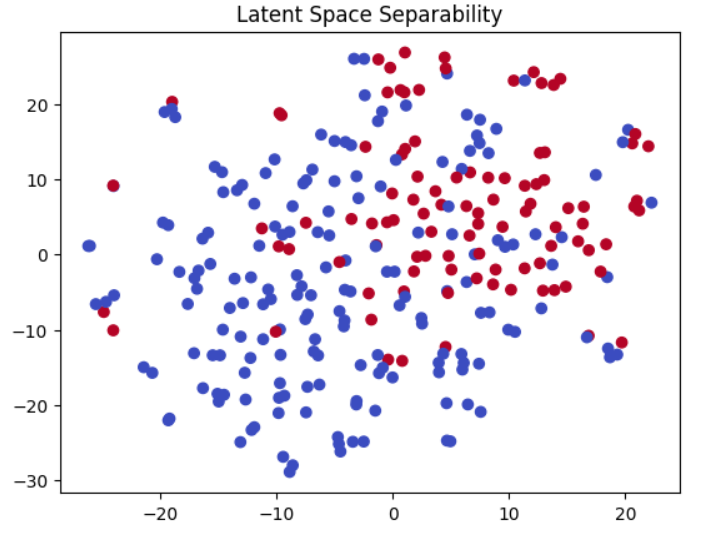
\includegraphics[width=0.45\textwidth]{latent_space_seperability.png}
    \caption{Two-dimensional t-SNE projection of fused latent representations, showing separability between benign and malignant samples.}
    \label{fig:tsne}
\end{figure}

A two-dimensional t-SNE projection of the fused latent space, shown in Fig.~\ref{fig:tsne}, reveals distinct clustering patterns between benign and malignant cases, confirming the discriminative quality of the learned representations.

\subsubsection{PCA-Based 3D Projection}

\begin{figure}
    \centering
    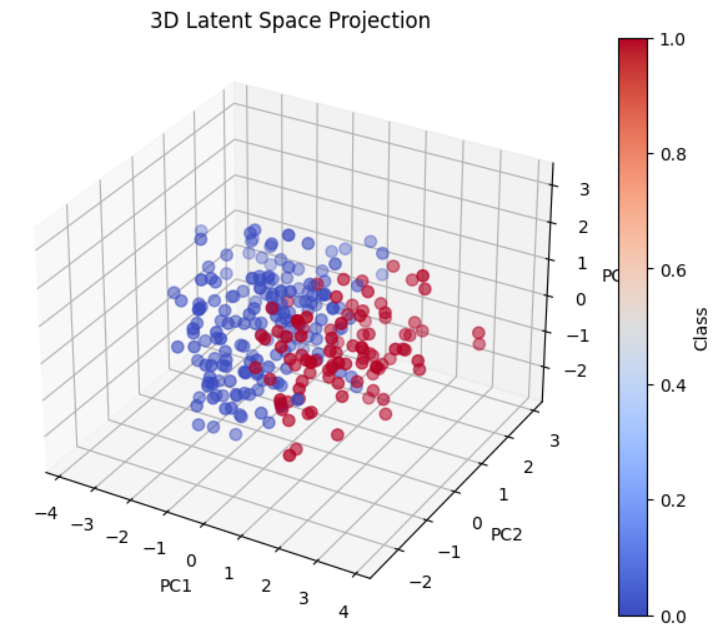
\includegraphics[width=0.45\textwidth]{3d_latent_space.png}
    \caption{Three-dimensional PCA projection of multimodal latent embeddings, illustrating class-wise separation across principal components.}
    \label{fig:pca3d}
\end{figure}

The three-dimensional PCA visualization in Fig.~\ref{fig:pca3d} further supports the observed class separability. The smooth transitions between clusters suggest that the model captures a continuous disease severity manifold rather than enforcing rigid class boundaries.

\subsection{Summary of Findings}
The experimental results demonstrate that the proposed multimodal latent fusion framework effectively integrates thermographic and mammographic information for breast cancer detection. The model achieves robust classification performance under noisy conditions, exhibits clear latent space separability, and provides interpretable decision explanations.

Collectively, these findings highlight the potential of latent-level multimodal fusion as a promising and interpretable approach for multimodal breast cancer analysis in research-oriented diagnostic settings.


\section{Conclusion and Future Work}
This work presented a multimodal breast cancer detection framework that integrates thermographic and mammographic information through latent-level feature fusion. Separate modality-specific encoders were employed to project high-dimensional features into a shared latent space, enabling effective alignment and reducing modality-induced representation gaps. The aligned latent embeddings were subsequently fused and utilized for classification.

Experimental results demonstrate that the proposed fusion approach achieves robust and stable classification performance, even under noisy input conditions. In addition, latent space visualizations using t-SNE and PCA confirm improved class separability, indicating that the learned representations effectively capture disease-related characteristics.

Beyond performance, this study emphasizes model interpretability through SHAP-based explainability analysis, providing insight into the latent features influencing prediction outcomes. This improves interpretability of the proposed framework.

Overall, the results suggest that latent-level multimodal fusion is a promising strategy for breast cancer detection, offering improved robustness, interpretability, and diagnostic reliability compared to unimodal approaches. Future work will focus on validating the framework on larger, clinically diverse datasets, incorporating explicit cross-modal attention mechanisms, and extending the model to support longitudinal and real-time diagnostic scenarios.


\bibliography{refs}
\bibliographystyle{IEEEtran}

\end{document}
